\chapter{Uživatelské rozhraní}

Vzhledem k tomu, že jádro emulátoru je architektonicky navrženo jako samostatná kompilační jednotka,
lze relativně jednoduše zkonstruovat hostovací grafické rozhraní pro systém, který podporuje \textit{C++20} standard, 
a který je odpovědný za vizualizaci a interakci s interním stavem emulátoru. 

Pro tyto účely bylo nutné správně navrhnout celkovou architekturu uživatelského grafického rozhraní tak, aby
co nejméně ovlivňovala rychlost emulace jádra \textit{PlayStation} sytému a aby také co nejrychleji
dokázala předávat informace o hostovacím vstupu jádru.
Jakožto cílové a testovací hostovací systémy jsem zvolil \textit{Windows} a \textit{Linux}.

\section{Použité technologie}

Podobně jako u jádra emulátoru, celková filozofie tohoto modulu stavěla na pilířích \textit{objektově orientovaného přístupu}, 
zkombinovanou s \textit{RAII} technologií, viz obrázek \ref{raii-heap-only}. Jelikož kompilace závisí na dvou naprosto odlišných
hostovacích systémech, bylo nutné zvolit multiplatformní knihovny, které se starají o správu okna a umožňují snadné
zobrazovaní pole pixelů na obrazovku.

Pro samotnou správu okna jsem zvolil knihovnu \textit{SDL2}, která nejenom umožňuje vykreslit obsah \textit{framebufferu} jádra systému,
ale dokáže zpracovat události zaslané z operačního systému, včetně práce s klávesovým vstupem a herních ovladačů.

Nicméně knihovna \textit{SDL2} neposkytuje žádné uživatelské grafické rozhraní. To je nucen vývojář napsat sám a tedy
bylo nutné hledat nadstavbu nad \textit{SDL2} knihovnou. Ta byla nalezena v knihovně \textit{Dear ImGui}, která nejenom
poskytuje uniformní grafické rozhraní, obsahující širokou škálu interaktivních objektů jako menu, tlačítka a vyskakující modální okna, jak můžeme vidět například v aplikaci Ship of Harkinian \ref{imgui-showcase}\footnote{Ship of Harkinian github: \url{https://github.com/will-pickett/ship-of-harkinian}},
ale celková filozofie této knihovny staví na \textit{immediate UI} filozofii, která zásadně zjednodušuje vývoj, prototypování a celkovou
správu grafického uživatelského rozhraní.

\begin{figure}[h]
	\centering
	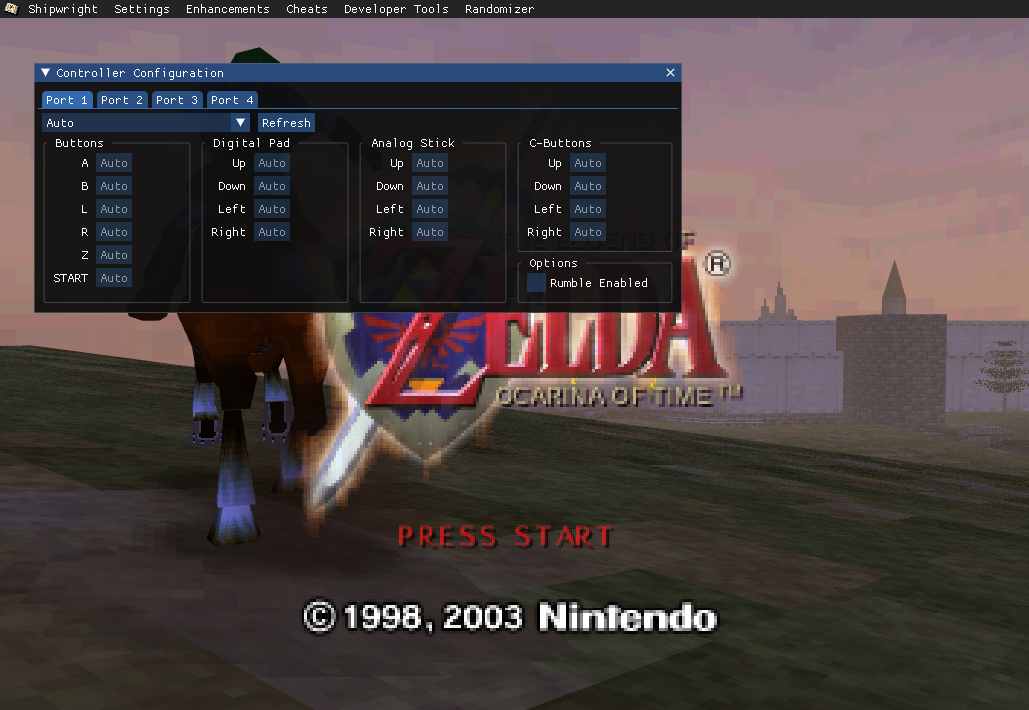
\includegraphics[width=1.0\textwidth]{obrazky-figures/soh.png}
	\caption[Příklad použití \textit{Dear ImGui}]{\textit{Dear ImGui} je velmi populární knihovna a poskytuje velmi jednoduchý způsob, jak zkonstruovat \textit{GUI}. V tomto obrázku
    můžeme vidět použití \textit{Menu} lišty, plovoucího okna, záložky, tlačítka, \textit{Drop-down} menu či přepínačů.}
	\label{imgui-showcase}
\end{figure}

\section{Architektura grafického rozhraní}

Celková architektura grafického uživatelského rozhraní je rozděleno na 3 části:\\[\baselineskip]
\begin{minipage}{\textwidth}
\begin{itemize}
    \item{\textbf{App} - objekt spravující okno, vykreslování, události z operačního systému a běh emulátoru.}
    \item{\textbf{Menu} - objekt spravující menu, tlačítka, \textit{GUI} a celkové ovládání jádra emulátoru.}
    \item{\textbf{Input} - objekt starající se nejenom o zasílání vstupu z hostovacího systému do jádra emulátoru, ale také zajišťuje přemapování jednotlivých tlačítek systému.}
\end{itemize}
\end{minipage}\\[\baselineskip]

\textit{App} objekt je implementován jako \textit{singleton} a figuruje jako vstupní bod do programu, viz obrázek \ref{frontend-arch-simple}. Detailnější propojení
pak můžeme vidět v obrázku \ref{frontend-arch-detailed}.

\begin{figure}[h]
	\centering
	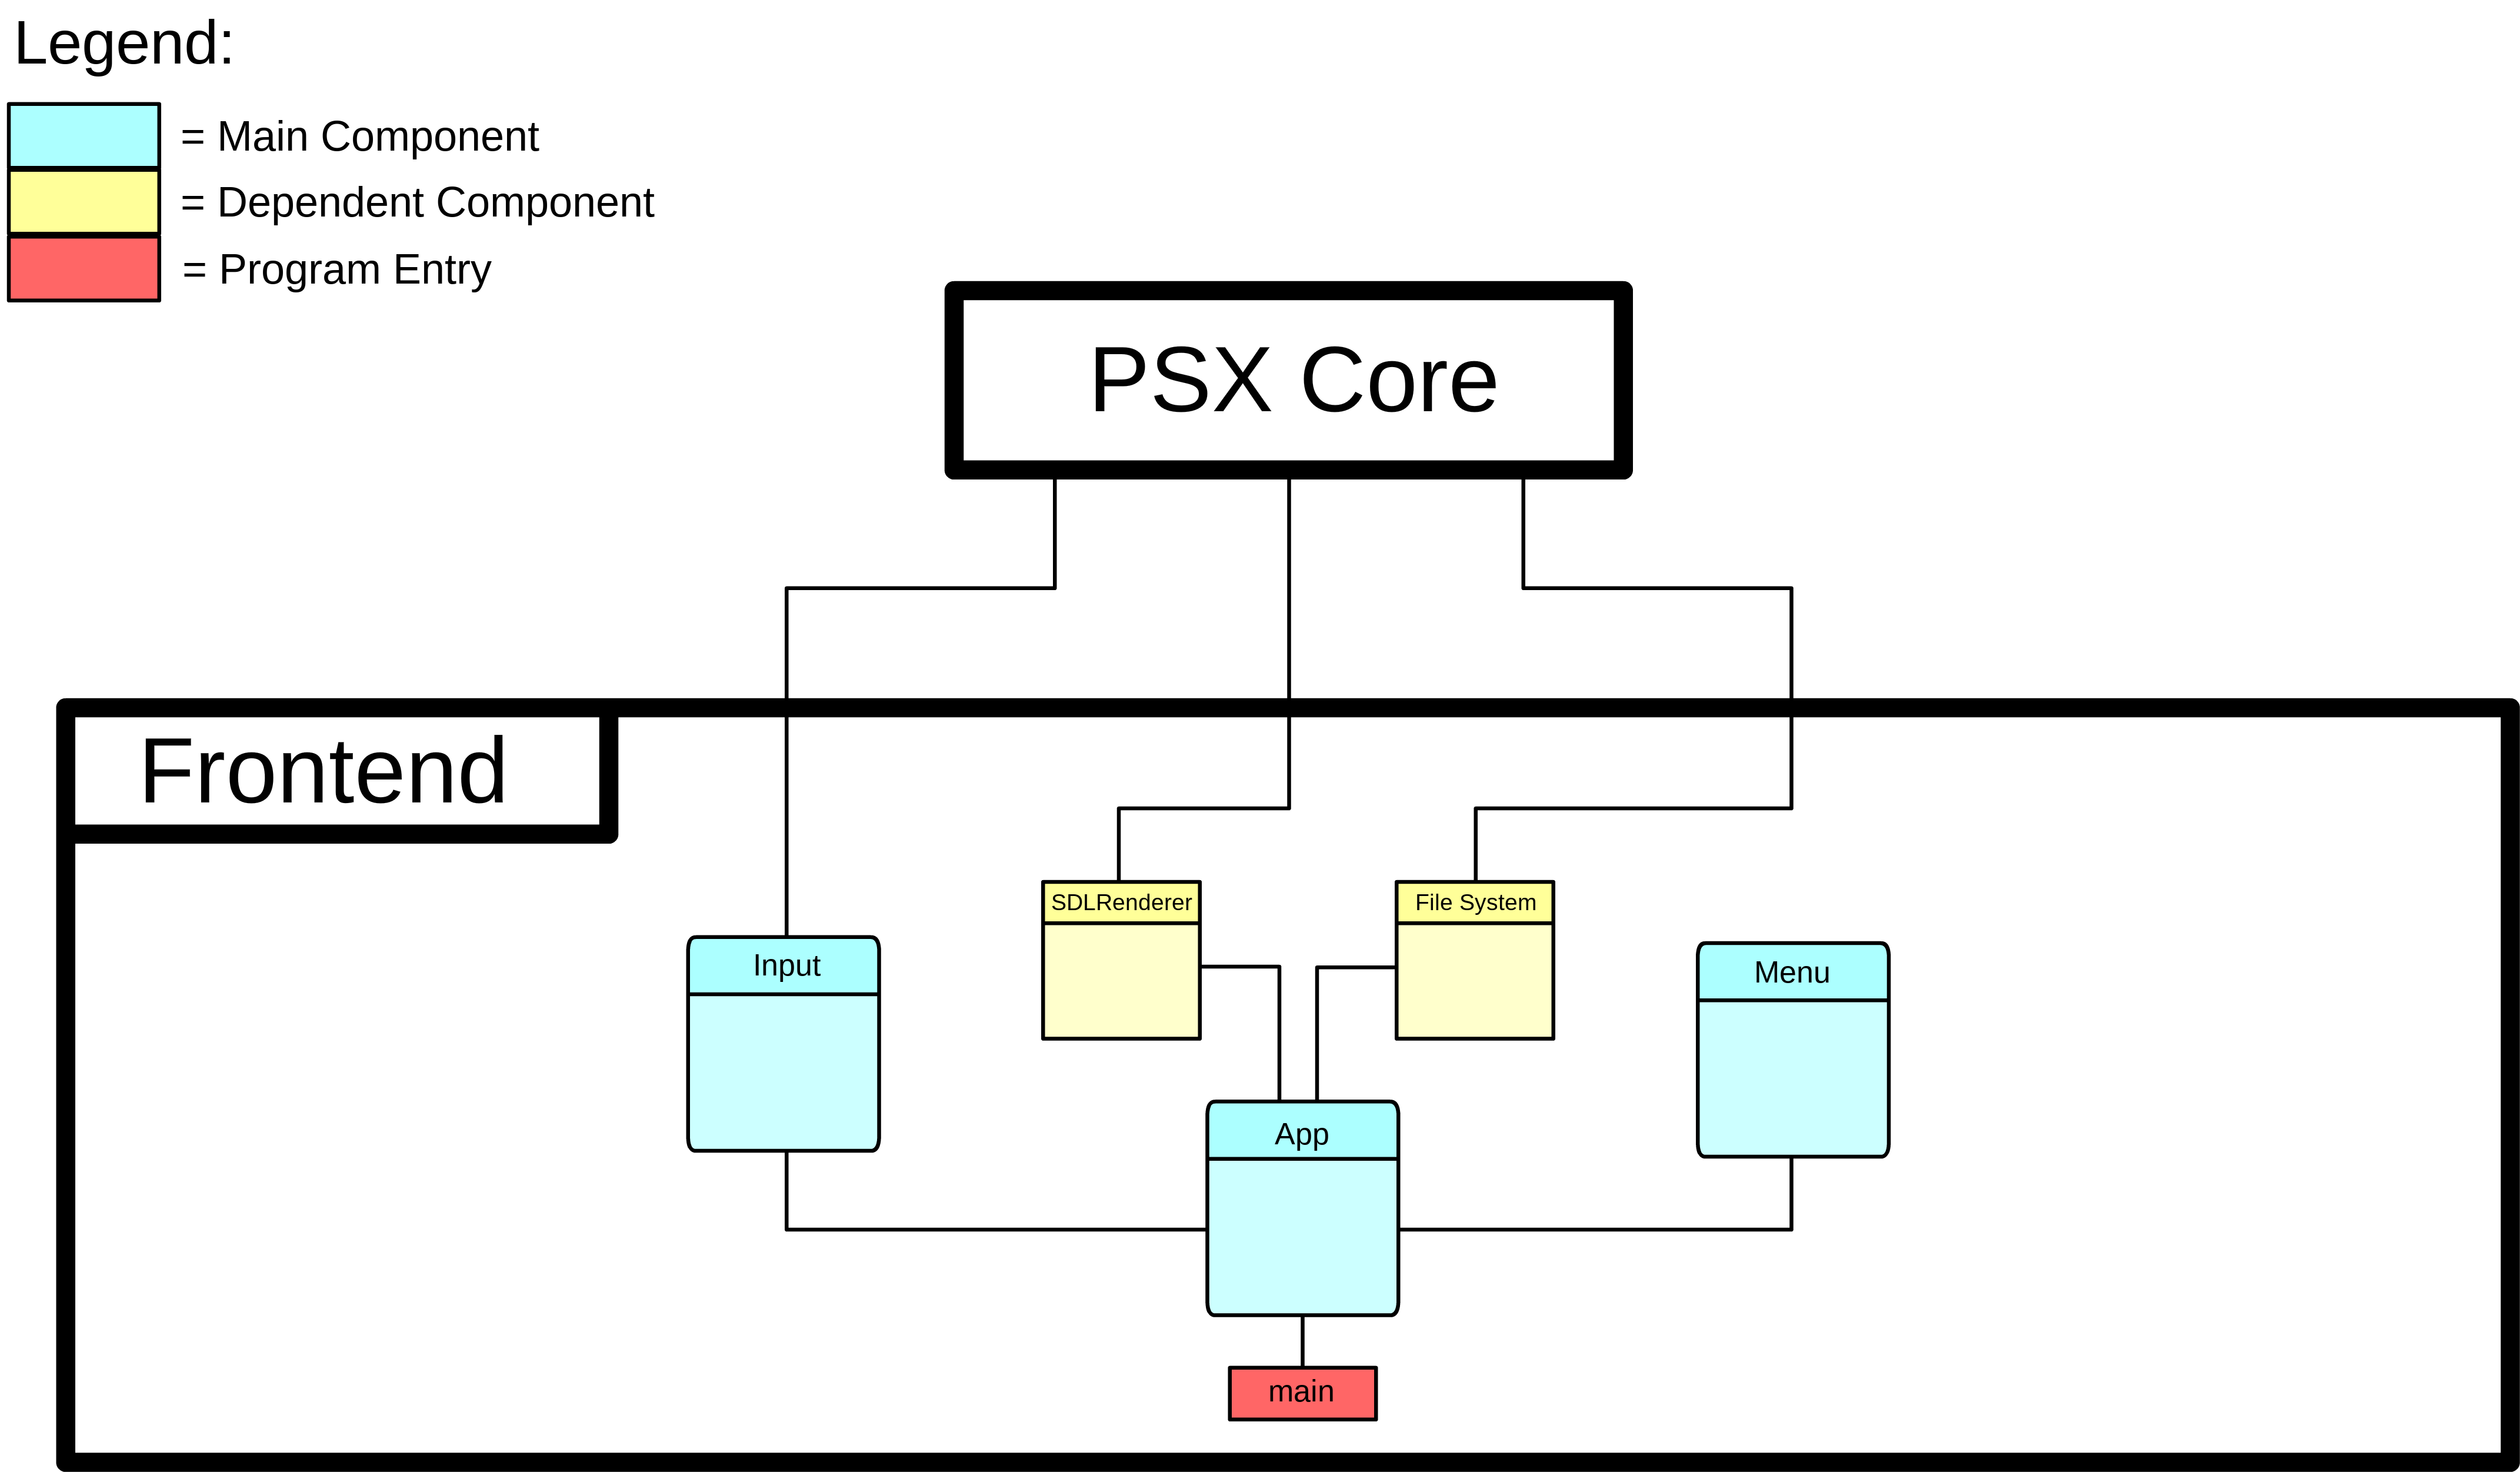
\includegraphics[width=1.0\textwidth]{obrazky-figures/frontend-arch-simple.png}
	\caption[Návrh architektury uživatelského rozhraní]{Vizualizace zapojení komponent uživatelského rozhraní. Jádro emulátoru komunikuje s uživatelském rozhraním a vzájemně si předávají zprávy. }
	\label{frontend-arch-simple}
\end{figure}

\begin{figure}[h]
	\centering
	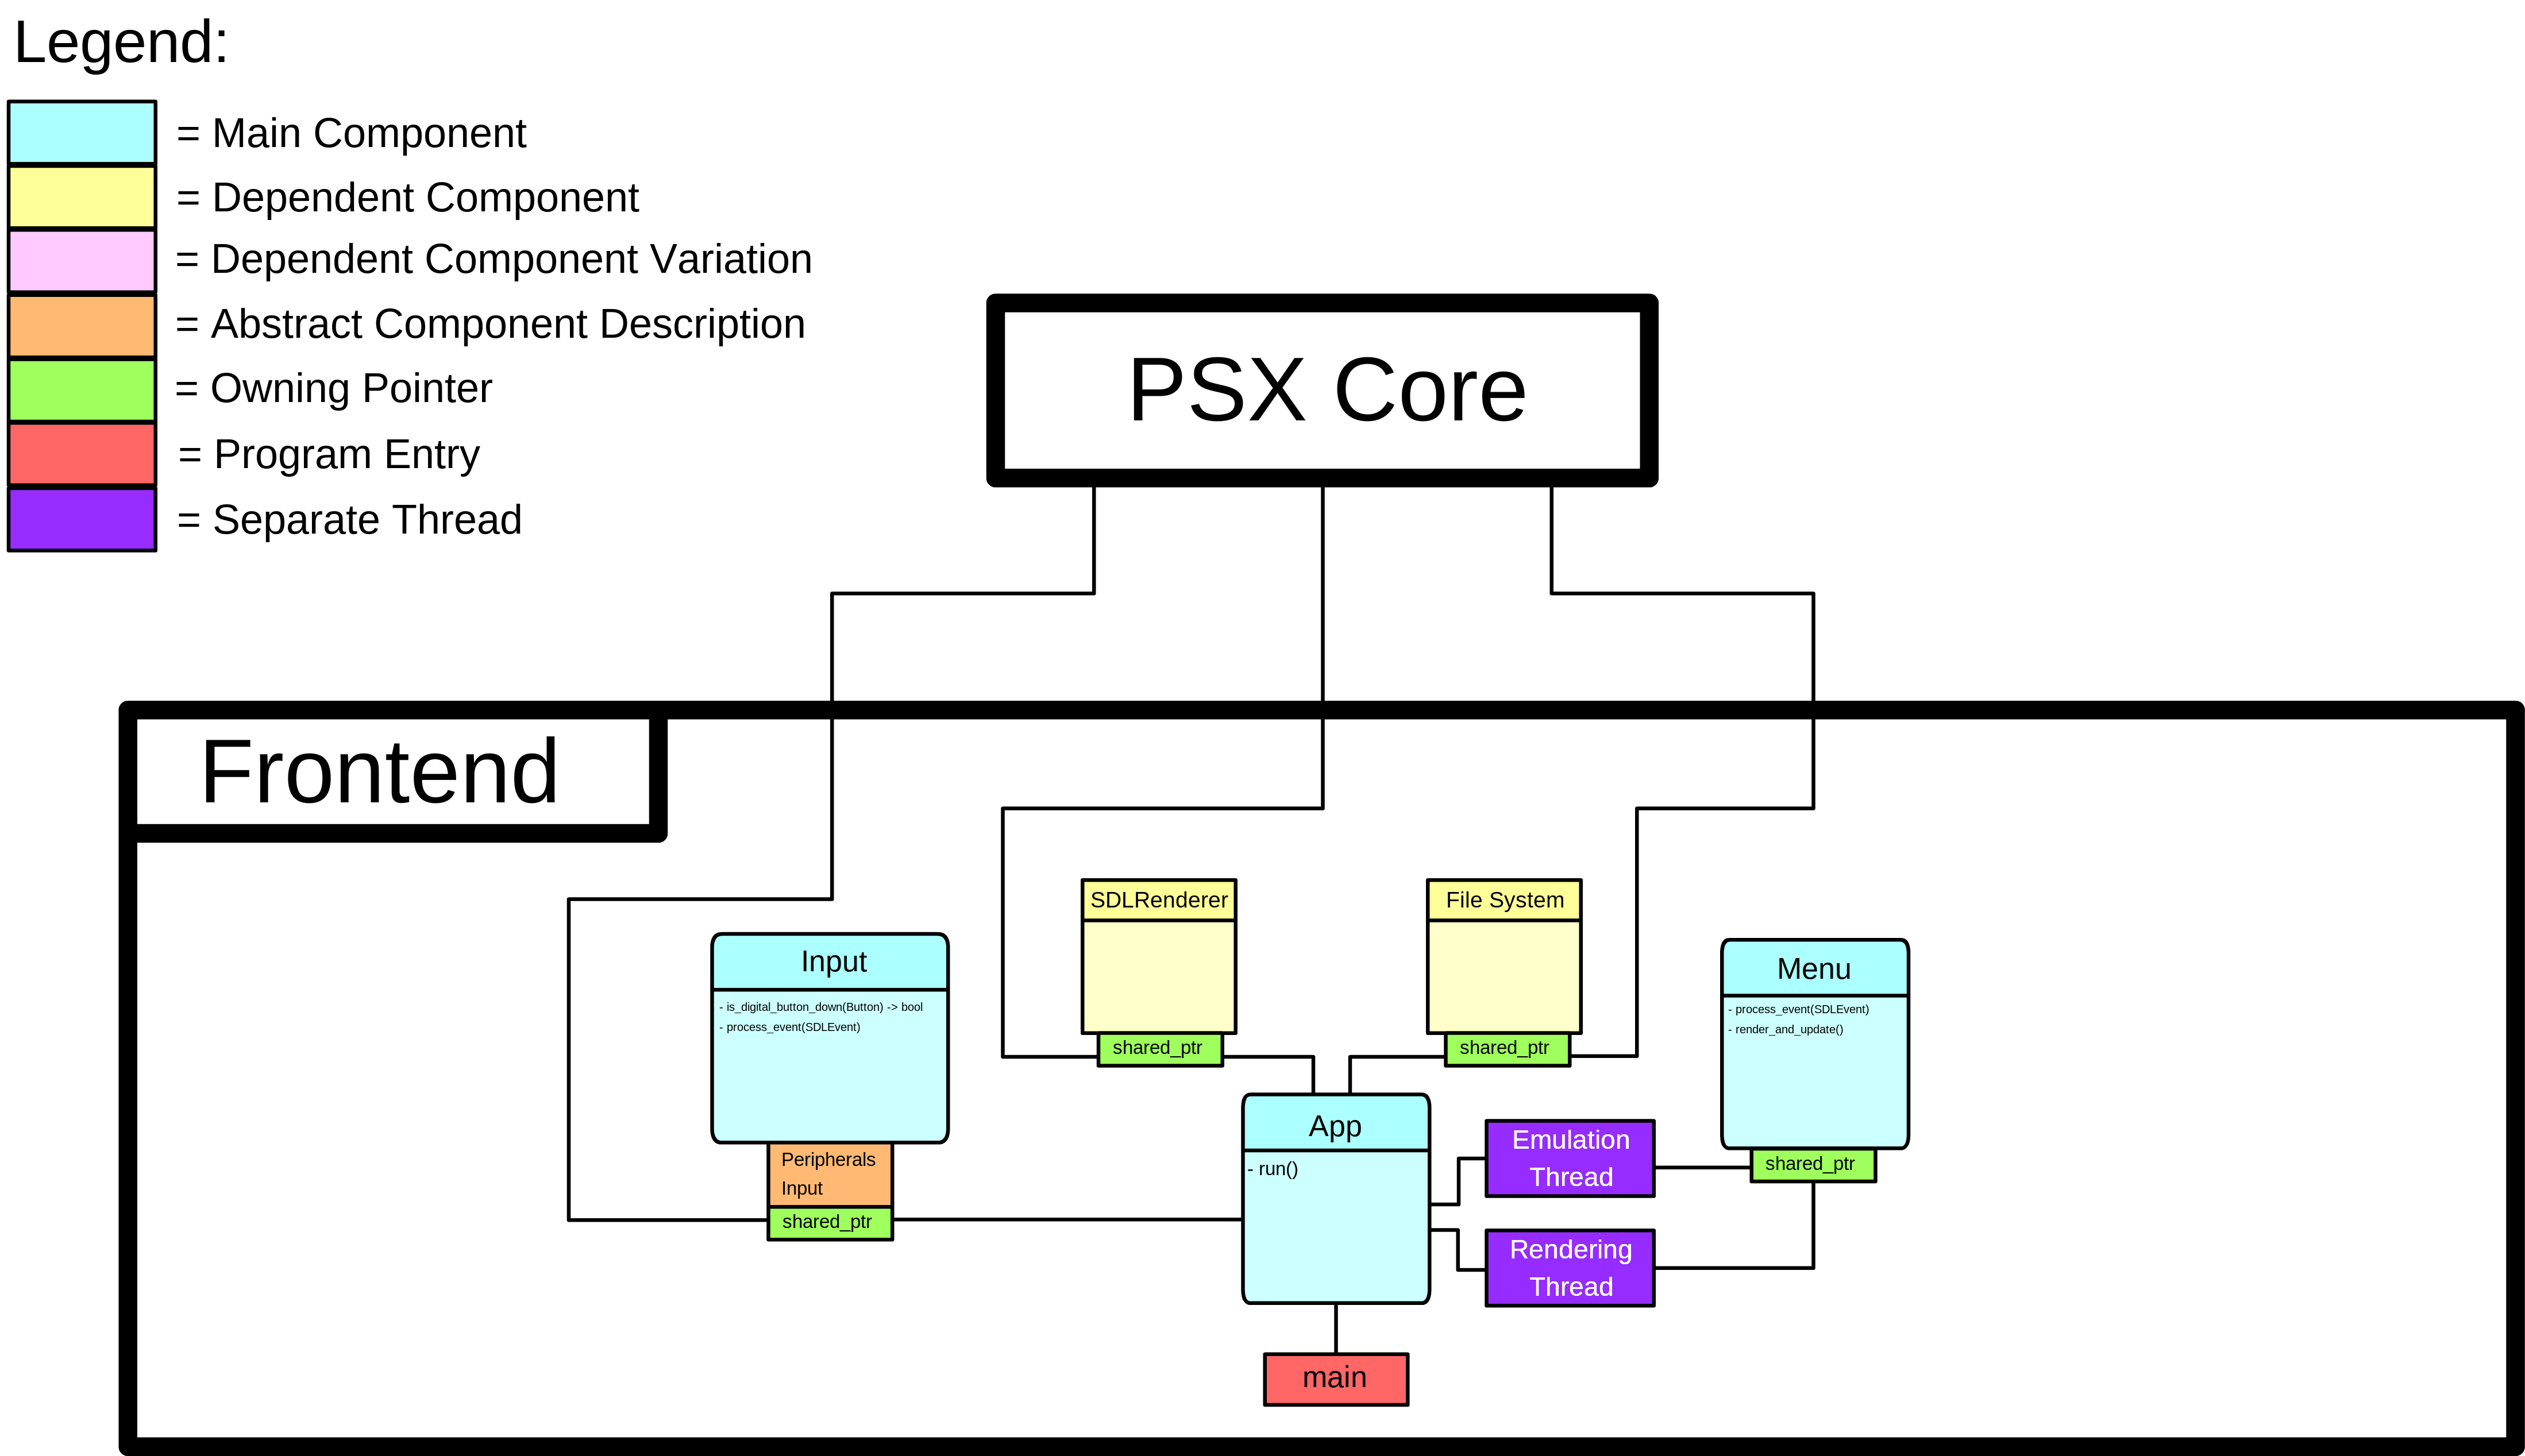
\includegraphics[width=1.0\textwidth]{obrazky-figures/frontend-arch-detailed.png}
	\caption[Detailní návrh architektury uživatelského rozhraní]{Aby uživatelské rozhraní mohlo zasílat informace o tlačítkovém vstupu, musí třída \textit{Input} podědit rozhraní \textit{PeripheralsInput} z jádra emulátoru.}
	\label{frontend-arch-detailed}
\end{figure}

\subsection{Vláknová architektura}

Pokud bychom chtěli emulovat \textit{PlayStation} systém v jednom vlákně, bezpochyby by to nebyl zásadní programovací problém. Popis fungování jedno-vláknové architektury je zachycen v obrázku \ref{single-threaded-arch}.

\begin{figure}[h]
	\centering
	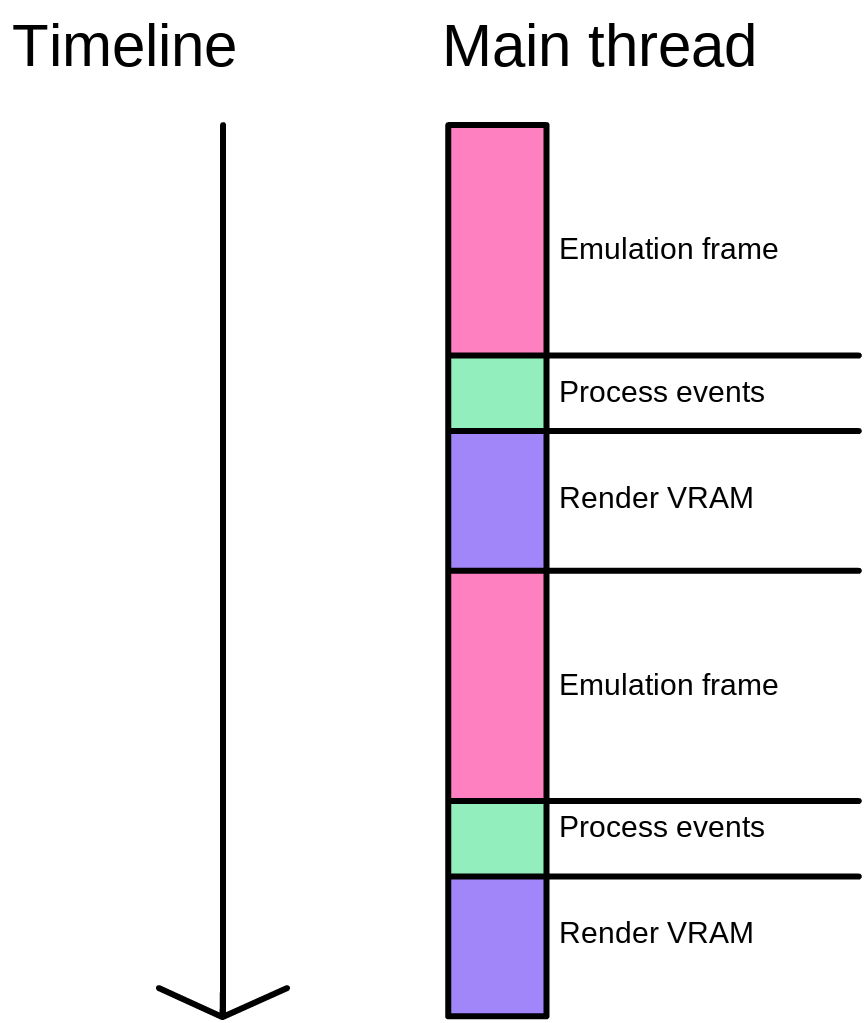
\includegraphics[width=0.5\textwidth]{obrazky-figures/frontend-arch-singlethreaded.png}
	\caption[Jedno-vláknová architektura emulátoru]{Jakmile se musí zpracovávat události z operačního systému, nebo se rendruje obsah paměti \textit{VRAM},
	emulace stojí.}
	\label{single-threaded-arch}
\end{figure}

Nicméně narazíme u tohoto návrhu na nepříjemnou věc. Zatímco se například vykresluje \textit{framebuffer}, nebo když se zpracovávají
události, či pokud zpracováváme menu, samotná emulace systému stojí. Jelikož je nám každý procesorový takt drahý, je třeba přesunout
emulační smyčku do separátního vlákna, jak můžeme vidět v obrázku \ref{double-threaded-arch}.

Aby toto bylo možné, hlavní vlákno a emulační vlákno si musí předávat informace o svém stavu a tudíž je nutné vytvořit komunikační a synchronizační
sekvence, ve kterých tyto dvě vlákna mohou bez problému komunikovat a navzájem se nezpomalovat. Tato dvou-vláknová architektura rozlišuje:

\begin{itemize}
	\item{\textbf{Renderovací} vlákno}
	\item{\textbf{Emulační} vlákno}
\end{itemize}

\textit{Emulační} vlákno se snaží co nejrychleji simulovat celý systém, dokud systém nevykreslí jeden snímek a nevystoupí do stavu \textit{VBlank}\footnote{Vertical blanking interval: \url{https://en.wikipedia.org/wiki/Vertical_blanking_interval}}.
To je signál pro \textit{Renderovací} vlákno, aby se probudilo a vyžádalo od \textit{Emulačního} vlákna obsah paměti \textit{VRAM} a informace
o tom, jak \textit{VRAM} vykreslit (např.: barevná hloubka \textit{VRAM}, ořezávací okno \textit{VRAM}, či zda-li je display zapnut).

Pro indikaci, zda-li nastal \textit{VBlank} a následné probuzení \textit{Renderovacího} vlákna je použita třída \textit{conditional\_variable} 
ze standardní knihovny \textit{C++}. Pokud probíhá kopírovaní \textit{VRAM} z \textit{Emulačního} vlákna do \textit{Renderovacího} vlákna,
celá procedura je ochráněna třídami \textit{mutex} a \textit{scoped\_lock}, které zajišťují exkluzivní přístup do kritické sekce.

Technicky vzato, exkluzivní kopírování \textit{VRAM} paměti mezi vlákny není bezpodmínečně nutné, ovšem zaplatíme za to tím, že výsledný obraz bude
vykazovat známky \textit{screen tearing}\footnote{Screen tearing: \url{https://en.wikipedia.org/wiki/Screen_tearing}}, kde část vykreslené \textit{VRAM} je z přechozího snímku a část ze snímku současného, vytvářející
artefakt, který může lidské oko rozptylovat.

\begin{figure}[h]
	\centering
	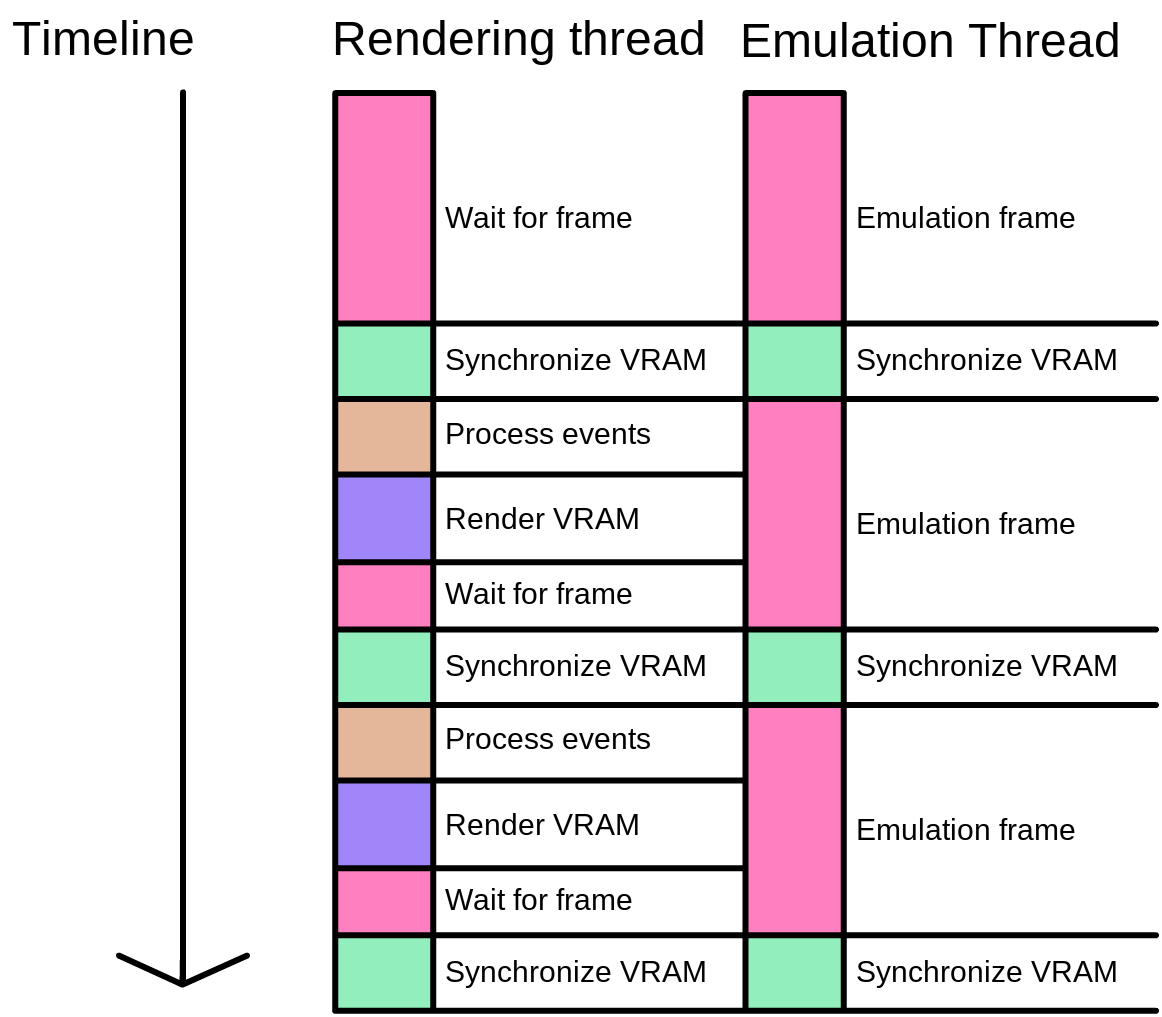
\includegraphics[width=0.6\textwidth]{obrazky-figures/frontend-arch-doublethreaded.png}
	\caption[Dvouvláknová architektura emulátoru]{I přesto, že dvou-vláknová architektura má určitou režii při komunikaci a výměně dat,
	emulace již není brzděna správou uživatelského rozhraní.}
	\label{double-threaded-arch}
\end{figure}

\subsection{Tlačítkový vstup}

Aby jádro emulátoru dokázalo přijímat vstup z hostovací klávesnice, či herního ovladače, musí nutně vystavit uživatelskému rozhraní rozhraní, které je nutné implementovat
na základě hostovacího systému. To znamená, že jádro emulátoru obsahuje čistě virtuální třídu, která je vyžadována při konstrukci emulátoru,
a která vyžaduje implementaci funkce \textit{is\_digital\_button\_down(DigitalButton)}, kde detail implementace samozřejmě závisí na hostujícím systému.

Jakmile uvnitř jádra započne \textit{Serial IO} komunikace s herním ovladačem, jádro vyžádá od uživatelského rozhraní nový stav
stisknutých kláves, či tlačítek ovladače. Tento přístup by měl minimalizovat artefakt známý jako \textit{input lag}. Moderní systémy pracují na 
principu zpracování událostí. V kombinaci hodinové komunikace s \textit{USB} perifériemi a navíc samotné zpracování vstupu uvnitř \textit{BIOSu} emulátoru, prodleva, 
která vznikne touto delegací má nemalou hodnotu. U testovaných her, tato prodleva činila 2-3 snímky.

Tento neduh je v emulačních kruzích dobře znám a existují složité procedury, který tento artefakt minimalizují (Například technika Run Ahead\footnote{RetroArch Run Ahead: \url{https://docs.libretro.com/guides/runahead/}}, implementovaná v emulačním frontendu RetroArch).

\section{Zobrazení obsahu VRAM}

Ačkoliv jsme architekturu výměny obsahu \textit{VRAM} zajistili synchronizačními objekty, samotné zobrazování obsahu \textit{VRAM} není snadná záležitost.
Jak bylo zmíněno, \textit{GPU} má 2 módy, jak interpretovat obsah \textit{VRAM} paměti: 

\begin{itemize}
    \item{sekvence \textbf{15-bitových} barev}
    \item{sekvence \textbf{24-bitových} barev}
\end{itemize}

Jelikož v \textit{SDL2} knihovně neexistuje způsob, jak měnit formát textury za běhu programu, je tedy nutno spravovat 2 textury se specifickými formáty,
do kterých emulátor kopíruje obsah \textit{VRAM}, a které se vykreslují do okna. Situaci nám taky komplikuje ten fakt, že \textit{GPU} specifikuje
ořezávací obdélník, pomocí něhož na obrazovce zobrazuje pouze specifickou část \textit{VRAM} paměti. Tento ořezávací obdélník závisí na interních registrech
\textit{GPU} a je netriviální jej vypočítat.

\section{Grafické uživatelské rozhraní (GUI)}

Jak bylo zmíněno, grafická část uživatelského rozhraní je řešena pomocí knihovny \textit{Dear ImGui}, přičemž interakce s vnitřním stavem emulátoru
je realizována přes \textit{Menu lištu}, která ve výchozím stavu je přítomna v horní části okna. Přes toto \textit{menu} má uživatel možnost
pozměnit a ovládat emulátor, viz obrázek \ref{gui-showcase}.

\subsection{Rozložení GUI}

Celkové \textit{GUI} je navrženo pro minimální obstrukci okna. \textit{Menu lišta} má celkem 4 položky:\\[\baselineskip]
\begin{minipage}{\textwidth}
\begin{itemize}
	\item{\textbf{State} - Položka pro reset, načítání a ukládání stavu emulátoru.}
	\item{\textbf{Controls} - Položka pro mapování hostových tlačítek na tlačítka digitálního ovladače \textit{PlayStation}.}
	\item{\textbf{Debug} - Položka pro užitečné debugovací funkce jako je vizualizace celé \textit{VRAM} či určení rychlosti emulace.}
	\item{\textbf{Hide} - Položka pro skrytí \textit{menu lišty}. Skryté \textit{menu} může být obnoveno pomocí klávesy \textit{ESC}.}
\end{itemize}
\end{minipage}\\[\baselineskip]

\begin{figure}[h]
	\centering
	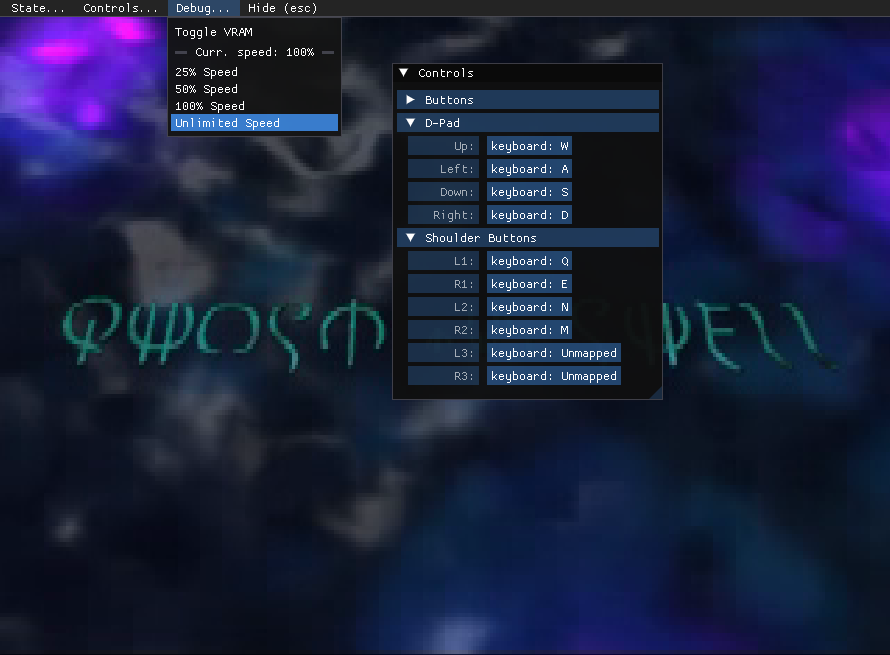
\includegraphics[width=1.0\textwidth]{obrazky-figures/gui-showcase.png}
	\caption[Grafické uživatelské rozhraní emulátoru]{\textit{GUI} emulátoru}
	\label{gui-showcase}
\end{figure}

\subsubsection{State}

Pro ovládání stavu emulátoru, uživatel má několik možností jak s emulátorem interagovat.
V prvém případě uživatel může resetovat stav konzole, kde systém spustí inicializační rutinu \textit{BIOSu} a začne
se spouštět hra od samého začátku.

Bohužel, v současném stavu emulátor nepodporuje ukládání postupu ve hře pomocí \textit{MemoryCard} periférie.
Tento nedostatek je řešen tak, že uživatel má možnost uložit celý stav emulátoru do souboru hostovacího systému.
Tím pádem je postup uložen i bez podpory \textit{MemoryCard} periférie.
Stejně jako uložení, emulátor podporuje načítání uloženého stavu.

\subsubsection{Controls}

Emulátor podporuje základní rozložení digitálního \textit{PlayStation} ovladače na klávesnici, přičemž počáteční rozložení mapování tlačítek je podchyceno v tabulce \ref{controls-map}.
\begin{table}[htbp]
    \caption{Základní mapa tlačítek}
    \begin{center}
    \begin{tabular}{ |c|c|c| }
    \hline
    \textbf{PlayStation ovladač} & \textbf{Klávesnice} \\
    \hline
    Select & L \\
    Start & K \\
    D-pad Up & W \\
    D-pad Right & D \\
    D-pad down & S \\
    D-pad left & A \\
    L2 & N \\
	R2 & M \\
    L1 & Q \\
    R1 & E \\
    Triangle & Arrow Up \\
    Circle & Arrow Right \\
    Cross & Arrow Down \\
    Square & Arrow Left \\
    \hline
    \end{tabular}
    \end{center}
    \label{controls-map}
\end{table}
Jelikož uživatel může mít specifickou klávesnici, či různé klávesové rozložení, je nutná implementace přemapování tlačítek.
Tato odpovědnost je řešena právě ve třídě \textit{Input}, kde se používá \textit{unordered\_map} ze standardní knihovny \textit{C++} pro správu jednotlivých přemapování.

U každého mapování uživatel může kliknout na specifickou klávesu kterou chce přemapovat.
To spustí modální okno které odposlouchává klávesový vstup, přičemž první stisknutá klávesa
po spuštění tohoto okna se bere jako mapovací klávesa. 

\subsubsection{Debug}

Aby člověk mohl pohlédnout za oponu a měl větší kontrolu nad chodem emulátoru, v menu existuje \textit{Debug} položka, ve které
si uživatel může zobrazit obsah celé \textit{VRAM} a má tak možnost vidět co se děje mimo vykreslený \textit{framebuffer}.
Stejně tak může uživatel nastavit rychlost chodu celého emulátoru a nastavovat změnu rozlišení.

\subsection{Prevence dark patterns}

Ač chtěně či nechtěně, může se stát že \textit{GUI} je architektonicky navržena tak, že části rozhraní dokáží svést uživatele k akcím
které provést vůbec nechtěl (tzv.: \textit{dark patterns/anti patterns\footnote{Dark pattern: \url{https://en.wikipedia.org/wiki/Dark_pattern} \newline Anti-pattern: \url{https://en.wikipedia.org/wiki/Anti-pattern}}}). Když bylo \textit{GUI} tohoto emulátoru testováno, ukázalo se, že uživatel při ukládání stavu emulátoru
mohl omylem kliknout na tlačítko \textit{Reset}, které bez upozornění systém obnovilo do původního stavu, přičemž vymazal jakýkoliv postup ve
hře, který se uživatel zrovna snažil uložit.

Z tohoto důvodu je třeba řešit prevence a záchranné sítě, které tomuto neduhu předejdou. V tomto případě \textit{Reset} tlačítko bylo odděleno oddělovací čárou,
klávesová zkratka pro reset systému byla odstraněna a při kliknutí na tlačítko \textit{Reset} se zobrazí modální okno, které se ptá na konfirmaci
uživatelské akce, viz obrázek \ref{reset-confirmation}.

\begin{figure}[hbt]
    \begin{subfigure}{0.5\textwidth}
        \centering
        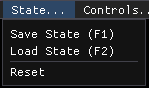
\includegraphics[width=0.9\textwidth, height=4cm]{obrazky-figures/reset-anti-pattern.png}
    \end{subfigure}
    \begin{subfigure}{0.5\textwidth}
        \centering
        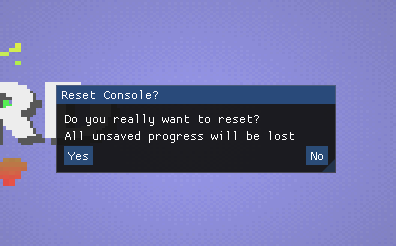
\includegraphics[width=0.9\textwidth, height=4cm]{obrazky-figures/reset-confirmation.png}
    \end{subfigure}
    \caption[Prevence \textit{dark-patterns/anti-patterns}]{Ačkoliv \textit{Reset} tlačítko je nebezpečně blízko \textit{Save State} a \textit{Load State} tlačítek,
    po jeho stisknutí vyskočí konfirmační okno, které jakýkoliv překlik neguje.}
    \label{reset-confirmation}
\end{figure}

\section{Spuštění programu}

Emulátor očekává své spuštění přes příkazovou řádku, kde mu uživatel musí specifikovat externí data, se kterými pak emulátor dokáže pracovat.
Pro minimální chod emulátoru je nutné předat cestu k \textit{BIOS} souboru v hostovacím systému jakožto první argument programu. Bez \textit{BIOSu} nebude emulátor schopen fungovat.
Emulátor byl testován na dvou verzích \textit{PlayStation BIOSu}:

\begin{itemize}
    \item{(md5sum: \textit{924e392ed05558ffdb115408c263dccf}) \textit{PSX BIOS} verze \textit{SCPH1001}}
    \item{(md5sum: \textit{c53ca5908936d412331790f4426c6c33}) modifikovaný \textit{PSX BIOS} pro \textit{PSP}}
\end{itemize}

Bohužel, jedná se o licencovaný software, a tedy \textit{BIOS} nemůže být distribuován spolu s emulátorem. Pro získání \textit{BIOSu} musí člověk
vlastnit originální konzoli a \textit{BIOS} z ní extrahovat. Tudíž ani stránky jako \textit{google}, či \textit{archive.org} nepomůžou. 

Ačkoliv emulátor pouze s \textit{BIOSem} poběží, je nutné specifikovat programu cestu k obrazu hry v hostovacím systému, pro
získání plného využití tohoto softwaru.
V současné době, tento emulátor podporuje pouze bitové kopie sektorů disku s jednou stopou. Nicméně některé hry
obsahovaly na disku více stop (ve většině případů se oddělovaly datové stopy a audio stopy). Tyto typy her
nejsou podporovány a ačkoliv lze načíst pouze datová stopa více-stopového disku, může se stát že hra vyžádá data
z jiných stop a tedy ukončí chod emulátoru.
Cestu k bitové kopii jedno-stopového \textit{PlayStation} disku je nutno specifikovat jako druhý argument programu.

Po specifikaci argumentů emulátor automaticky načte \textit{BIOS} i \textit{Disk} a okamžitě
začne systém emulovat.